\documentclass[12pt]{article}
\usepackage[margin=1in]{geometry}
\usepackage{graphicx}
\usepackage{booktabs}
\usepackage{amsmath}
\usepackage{hyperref}

\title{Replicating Group Average Treatment Effects from Knaus (2022)}
\author{Hunter Massey}
\date{\today}

\begin{document}
\maketitle

\section{The Original Paper}

This project replicates one result from Michael C. Knaus's paper, ``Double machine learning-based programme evaluation under unconfoundedness,'' published in \textit{The Econometrics Journal}. The paper studies Swiss Active Labour Market Policy programs and asks how different training programs affect later employment outcomes. The paper is an example of causal machine learning: machine learning is used to estimate nuisance functions, but the final goal is causal estimation rather than prediction.

The empirical framework assumes unconfoundedness: after conditioning on observed covariates, assignment to different labor market programs can be treated as independent of potential outcomes. Under that assumption, the paper uses double machine learning with doubly robust scores to estimate average, subgroup, and individualized treatment effects.

\section{The Result of Interest}

The target result is Table 4 of Knaus (2022), which reports group average treatment effects for four active labor market programs relative to nonparticipation. The table studies heterogeneity by gender, foreigner status, and employability. I focus on this table because it is a clear application of the core DML idea from class: first construct a doubly robust pseudo-outcome, then run standard regressions on that pseudo-outcome to summarize treatment-effect heterogeneity.

\section{Data and Methods}

The data come from the restricted-use Swiss Active Labour Market Policy dataset distributed through SwissUbase/FORSbase. Because the data are restricted, the raw file is not included in the GitHub repository. The repository includes instructions for placing the raw CSV file in the \texttt{input/} folder before running the replication.

The preprocessing script reads the raw data, keeps the German-speaking canton sample, removes the employment and personality treatment categories, constructs the 45 covariates used in the replication, assigns pseudo-start dates to the no-program group, removes observations already employed before the relevant start point, and constructs the outcome. The outcome is the number of months employed over a 31-month window after the treatment or pseudo-treatment start.

The DML equation used in the paper is the doubly robust score for the average potential outcome:
\[
\hat{\Gamma}_{i,w}
=
\hat{\mu}(w, X_i)
+
\frac{D_i(w)\left(Y_i - \hat{\mu}(w, X_i)\right)}
{\hat{e}_w(X_i)}.
\]
Here, $\hat{\mu}(w,X_i)$ is the predicted outcome under treatment $w$ and $\hat{e}_w(X_i)$ is the predicted probability of receiving treatment $w$. In class terms, these are nuisance functions. DML uses machine learning to estimate them, but the doubly robust score protects the treatment-effect estimate from moderate first-stage prediction errors.

For Table 4, the relevant pseudo-outcome is the difference between two APO scores:
\[
\hat{\Delta}_{i,w,w'} = \hat{\Gamma}_{i,w} - \hat{\Gamma}_{i,w'}.
\]
I then regress this treatment-effect pseudo-outcome on subgroup indicators for female, foreigner, and employability. This is why the final subgroup regressions look like ordinary OLS regressions, even though the dependent variable is a causal treatment-effect score.

\section{Replication Results}

\begin{figure}[h]
\centering
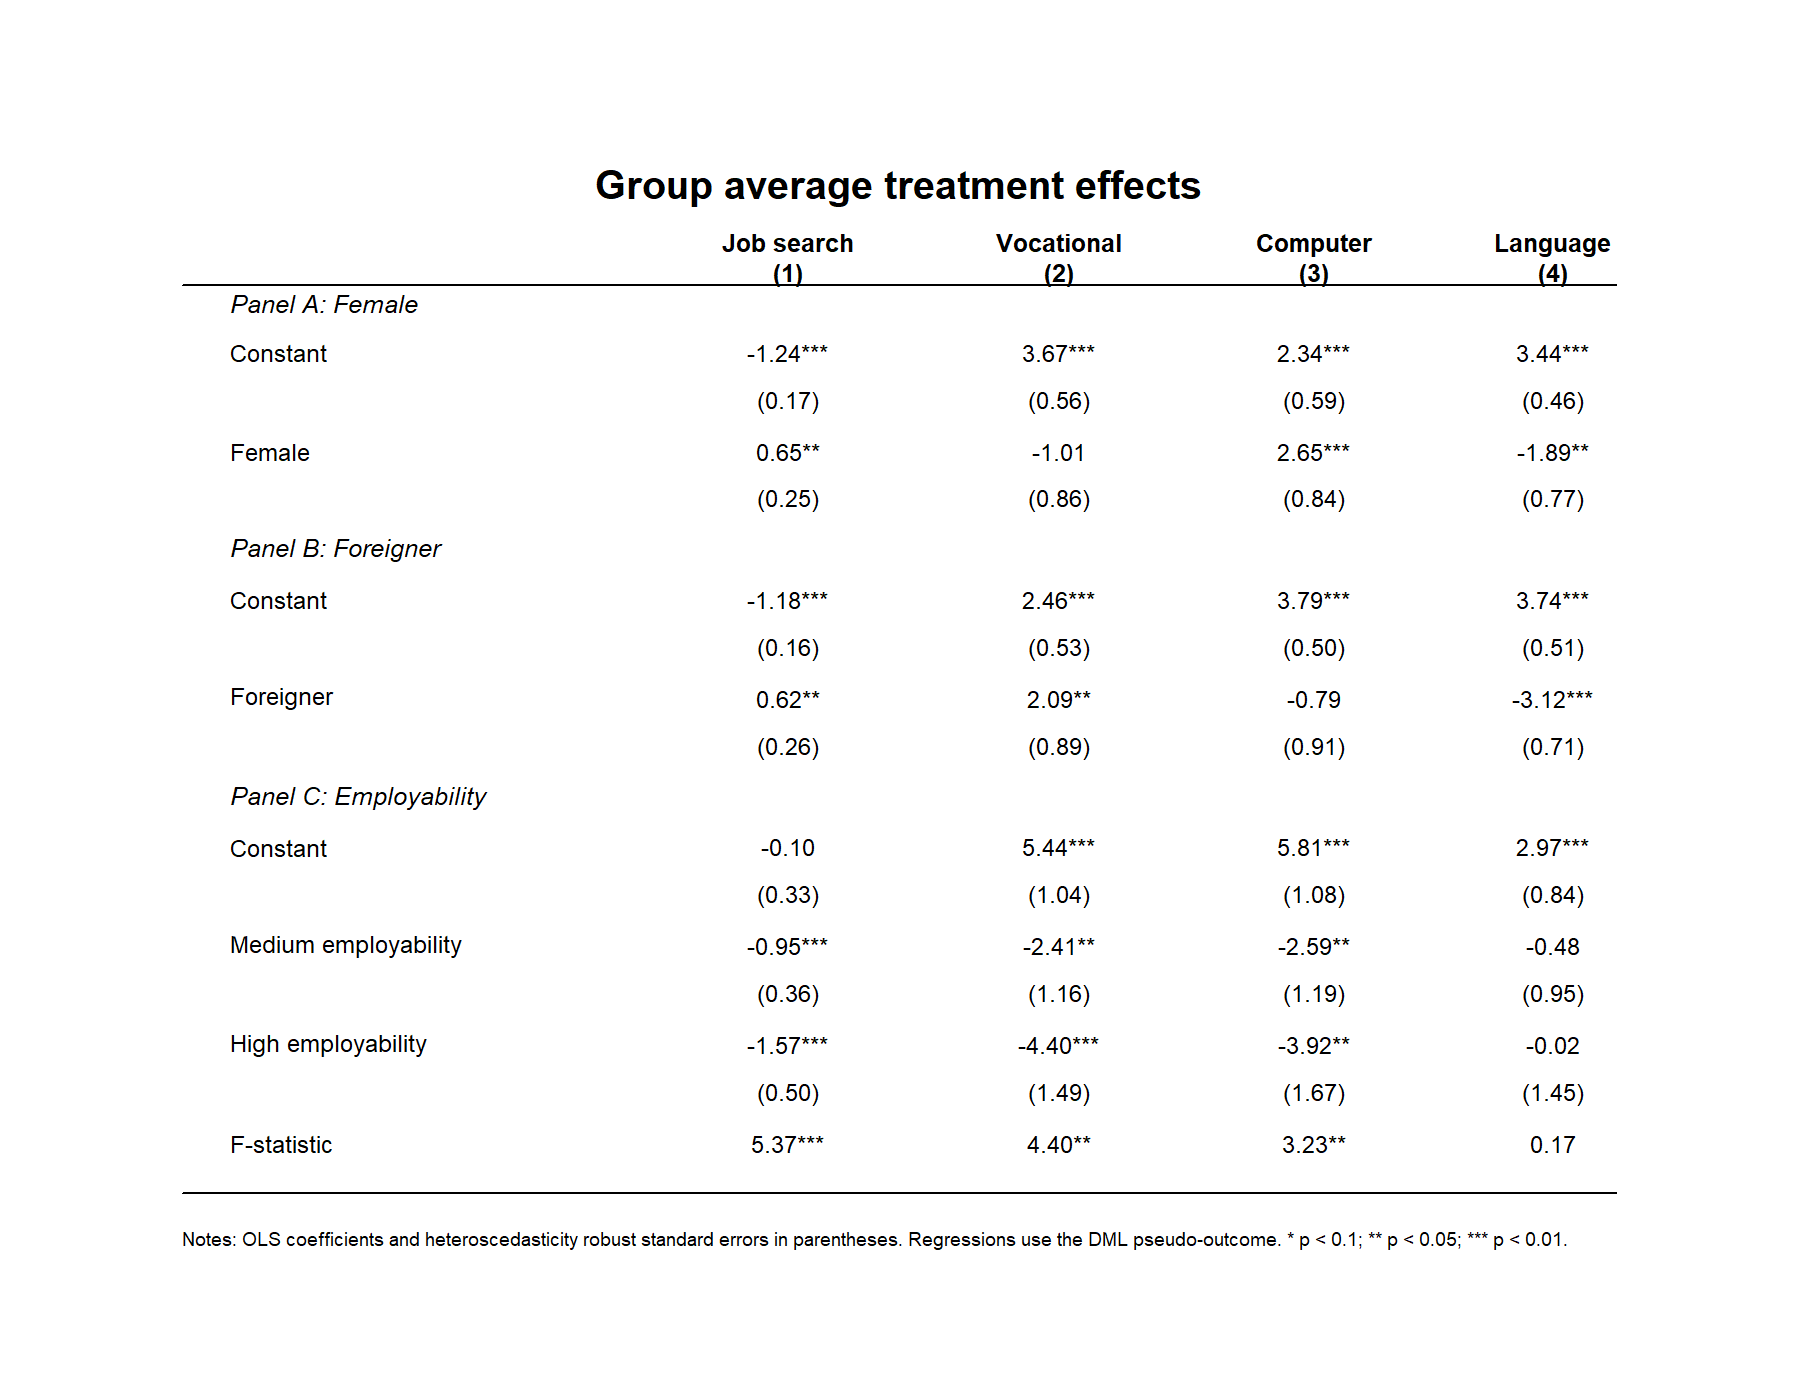
\includegraphics[width=0.95\textwidth]{../output/figures/table4_replication_output.png}
\caption{Replication of Table 4: Group average treatment effects}
\label{fig:table4rep}
\end{figure}



The replicated table closely matches the structure and broad findings of the published table. Job search training is generally negative relative to no program, while vocational, computer, and language programs are generally positive. The subgroup patterns also line up with the paper: women benefit relatively more from computer training and less from language courses; foreigners benefit more from vocational training but less from language courses; and lower-employability workers generally gain more from the hard-skill programs.

The replication is not expected to match the paper exactly. I use generalized random forests with fixed tuning parameters to make the computation feasible on a laptop, while the paper uses fully tuned honest random forests. The cleaned sample size is also slightly different because the no-program group requires a simulated pseudo-start date. These two differences explain the remaining numerical gap.

\section{What I Learned}

The easiest part of the replication was understanding the second-stage analysis once the DML pseudo-outcome was available. The logic is very close to what we learned in class: estimate the nuisance functions, form the doubly robust score, and then use ordinary statistical tools on that score.

The hardest part was data preparation. The raw data are restricted, and the original full data-preparation script was not included in the files I had. The no-program group required a pseudo-start simulation, and small changes in that step change the final sample size. This made the replication a useful lesson in how much causal machine learning still depends on careful data construction before any machine learning model is run.

If I were preparing this paper for replication by others, I would include a fully automated preprocessing script and a smaller cached version of the cleaned analysis data. That would make the DML part much easier to verify and would reduce ambiguity about sample restrictions.

\begin{thebibliography}{9}
\bibitem{knaus2022}
Knaus, Michael C. 2022. ``Double machine learning-based programme evaluation under unconfoundedness.'' \textit{The Econometrics Journal} 25(3): 602--627.
\end{thebibliography}

\end{document}
